%=====================================================================
%  07-NEGATIVE-ENTROPY.TEX — NEGATIVE ENTROPY (CERF & ADAMI)
%=====================================================================
%  Sumber utama: Cerf & Adami, "Negative entropy in quantum
%  information theory" (1997). Perbaikan notasi dari versi lama:
%    * \rho{A|B}         -> \rho_{A|B}
%    * (1_A\bigotimes\rho_B)^{-1} -> (I_A\otimes\rho_B^{-1})
%    * \ket{...}){AB}    -> subskrip _{AB} yang benar
%=====================================================================
\section{NEGATIVE ENTROPY}

%---------------------------------------------------------------------
%  INTRODUCTION 1 — gambaran umum teori informasi kuantum
%---------------------------------------------------------------------
\begin{frame}
    \frametitle{INTRODUCTION 1}
    \vspace*{-0.5cm}
    \begin{columns}[T]
        \begin{column}{0.5\textwidth}
            \begin{itemize}\tiny\justifying
                \item \textbf{Deskripsi Umum Quantum Information Theory}
                    \begin{itemize}\tiny\justifying
                        \item[$\Rightarrow$] Memberikan deskripsi konsisten tentang
                            \textit{entanglement} kuantum.
                        \item[$\Rightarrow$] Paralel dengan teori informasi klasik
                            (Shannon) namun berbasis sepenuhnya pada matriks densitas.
                    \end{itemize}
                \item \textbf{Perbedaan dengan Teori Shannon}
                    \begin{itemize}\tiny\justifying
                        \item[$\Rightarrow$] Berfokus pada matriks densitas, bukan
                            distribusi probabilitas seperti dalam teori Shannon.
                        \item[$\Rightarrow$] Menemukan bahwa entropi kondisional bisa
                            negatif pada sistem terkait kuantum, seperti pasangan
                            Einstein--Podolsky--Rosen (EPR).
                    \end{itemize}
                \item \textbf{Penggunaan Density Matrices}
                    \begin{itemize}\tiny\justifying
                        \item[$\Rightarrow$] Entropi kuantum bernilai negatif dapat
                            ditelusuri ke matriks densitas kondisional yang memiliki
                            nilai eigen lebih besar dari satu.
                        \item[$\Rightarrow$] Menggunakan \textit{mutual} density matrix
                            untuk mendefinisikan \textit{mutual quantum entropy} atau
                            \textit{mutual entanglement}.
                    \end{itemize}
            \end{itemize}
        \end{column}

        \begin{column}{0.5\textwidth}
            \begin{itemize}\tiny\justifying
                \item \textbf{Hubungan Korelasi Klasik \& Entanglement Kuantum}
                    \begin{itemize}\tiny\justifying
                        \item[$\Rightarrow$] Penjelasan terpadu tentang korelasi klasik
                            dan \textit{entanglement} kuantum.
                        \item[$\Rightarrow$] \textit{Entanglement} kuantum dapat dianggap
                            sebagai \textit{super-korelasi} yang menghasilkan korelasi
                            klasik saat mempertimbangkan sistem ternary atau lebih besar.
                    \end{itemize}
                \item \textbf{Implikasi Quantum Information Theory}
                    \begin{itemize}\tiny\justifying
                        \item[$\Rightarrow$] Implikasi potensial terhadap fondasi
                            konseptual mekanika kuantum.
                        \item[$\Rightarrow$] Dasar pemahaman yang tepat untuk bidang baru:
                            komputasi kuantum, komunikasi kuantum, dan kriptografi kuantum.
                    \end{itemize}
                \item \textbf{Tantangan Quantum Information Processing}
                    \begin{itemize}\tiny\justifying
                        \item[$\Rightarrow$] \textit{Quantum information processing}
                            melibatkan qubit (bukan bit klasik) dengan hukum kuantum
                            yang berbeda.
                        \item[$\Rightarrow$] Qubit dapat berada dalam superposisi
                            kuantum --- konsep yang sepenuhnya berbeda dari mekanika klasik.
                    \end{itemize}
            \end{itemize}
        \end{column}
    \end{columns}
\end{frame}

%---------------------------------------------------------------------
%  INTRODUCTION 2 — matriks densitas kondisional (notasi diperbaiki)
%---------------------------------------------------------------------
\begin{frame}
    \frametitle{INTRODUCTION 2}
    \vspace*{-0.5cm}
    \begin{columns}[T]
        \small
        \begin{column}{0.5\textwidth}
            \begin{itemize}\tiny\justifying
                \item \textbf{Sifat Density Matrices dan Entropi von Neumann}
                    \begin{itemize}\tiny\justifying
                        \item[$\Rightarrow$] Matriks densitas, Persamaan~\ref{eq:matriks-densitas},
                            adalah konstruksi matematika sentral dalam teori informasi kuantum.
                        \item[$\Rightarrow$] Entropi von Neumann,
                            Persamaan~\ref{eq:entropi-vonneumann}, terkait dengan entropi
                            Boltzmann--Gibbs--Shannon, Persamaan~\ref{eq:entropi-bgs},
                            pada situasi klasik tertentu.
                    \end{itemize}
                \item \textbf{Analogi dengan Teori Informasi Klasik}
                    \begin{itemize}\tiny\justifying
                        \item[$\Rightarrow$] Konsep probabilitas kondisional
                            $p(x|y)=p(x,y)/p(y)$ pada teori klasik beranalogi dengan
                            matriks densitas kondisional
                            Persamaan~\ref{eq:rho-kondisional}.
                        \item[$\Rightarrow$] Teori informasi kuantum mempertahankan fasa
                            kuantum dengan menggabungkan probabilitas kuantum ke dalam
                            kerangka matriks densitas.
                    \end{itemize}
            \end{itemize}
        \end{column}

        \begin{column}{0.5\textwidth}
            \begin{itemize}\tiny\justifying
                \item \textbf{Matriks Densitas Kondisional}
                    \begin{equation}
                        \rho_{A|B}=\rho_{AB}\left(I_A\otimes\rho_B^{-1}\right)
                        \label{eq:rho-kondisional}
                    \end{equation}
                    \item[$\Rightarrow$] Dari Persamaan~\ref{eq:rho-kondisional},
                        entropi kondisional kuantum didefinisikan sebagai
                    \begin{equation}
                        S(A|B)=-\Tr\left(\rho_{AB}\log\rho_{A|B}\right)
                        = S(AB)-S(B).
                    \end{equation}
                    \item[$\Rightarrow$] Nilai eigen $\rho_{A|B}$ yang melebihi satu
                        menghasilkan $S(A|B)<0$ --- ciri khas sistem
                        ter-\textit{entanglement} \cite{cerf1997negative}.
            \end{itemize}
        \end{column}
    \end{columns}
\end{frame}

%---------------------------------------------------------------------
%  CORRELATION VERSUS ENTANGLEMENT 1 — EPR triplet
%---------------------------------------------------------------------
\begin{frame}
    \frametitle{CORRELATION VERSUS ENTANGLEMENT 1}
    \vspace*{-0.5cm}
    \begin{columns}[T]
        \begin{column}{0.5\textwidth}
            \begin{figure}
                \centering
                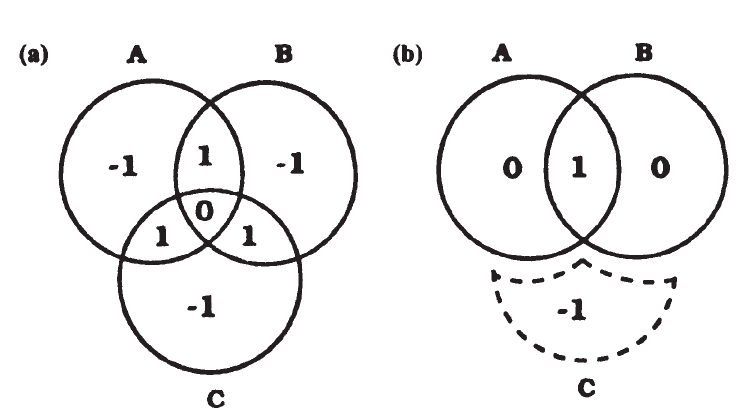
\includegraphics[width=\textwidth]{gambar/DIAGRAM/EPR-Triplet.png}
                \captionsetup{font=tiny, justification=justified, width=\textwidth}
                \captionof{figure}{(a) Diagram entropi ternary untuk sebuah
                ``EPR triplet''. (b) Diagram entropi subsistem AB tanpa kondisi
                pada C.}
                \label{fig:epr-triplet}
            \end{figure}
            \begin{itemize}\tiny\justifying
                \vspace{-0.6cm}
                \item[$\Rightarrow$] Fungsi Negative Conditional Entropy \\
                    Pada sistem kuantum komposit, entropi kondisional negatif
                    memberi pemahaman baru tentang pembentukan korelasi klasik
                    dari \textit{quantum entanglement}.
            \end{itemize}
        \end{column}

        \begin{column}{0.5\textwidth}
            \begin{itemize}\tiny\justifying
                \item[$\Rightarrow$] Sistem EPR-triplet \\
                    Tinjau sistem tiga partikel ABC dalam keadaan GHZ
                    (\textit{EPR-triplet})
                    \begin{equation}
                        \ket{\psi_{ABC}}=\frac{1}{\sqrt{2}}\left(\ket{000}+\ket{111}\right).
                    \end{equation}
                \item[$\Rightarrow$] Entangled state \\
                    Keadaan murni (\textit{entangled}) memiliki entropi gabungan
                    $S(ABC)=0$; diagram entropi ternary ABC
                    (Gambar~\ref{fig:epr-triplet}) menunjukkan \textit{ternary
                    mutual entropy}
                    \begin{equation}
                        \begin{aligned}
                            S(A{:}B{:}C)=\; & S(A)+S(B)+S(C)\\
                            & -S(AB)-S(AC)-S(BC)+S(ABC)
                        \end{aligned}
                    \end{equation}
                    menghilang --- hal umum untuk sistem tiga partikel yang
                    sepenuhnya ter-\textit{entangled}.
                \item[$\Rightarrow$] Density matrix subsistem AB \\
                    Melacak derajat kebebasan C memberikan matriks densitas
                    marginal subsistem AB,
                    Persamaan~\ref{eq:matriks-densitas-AB}, yang sesuai dengan
                    sistem klasik yang berkorelasi.
            \end{itemize}
        \end{column}
    \end{columns}
\end{frame}

%---------------------------------------------------------------------
%  CORRELATION VERSUS ENTANGLEMENT 2 — interpretasi pengukuran
%---------------------------------------------------------------------
\begin{frame}
    \frametitle{CORRELATION VERSUS ENTANGLEMENT 2}
    \vspace*{-0.5cm}
    \begin{columns}[T]
        \begin{column}{0.5\textwidth}
            \begin{itemize}\tiny\justifying
                \item[$\Rightarrow$] Teori Shannon \\
                    Mengabaikan keberadaan C, A dan B berkorelasi dalam arti
                    teori Shannon: subsistem AB menjadi tak terbedakan dari
                    himpunan statistik dengan jumlah seimbang keadaan
                    $\ket{100}$ dan $\ket{111}$.
                \item[$\Rightarrow$] Tracing Over \\
                    Operasi \textit{tracing over} menggambarkan terciptanya
                    korelasi klasik dari \textit{quantum entanglement}; penting
                    dalam deskripsi proses pengukuran: A dan B mewakili dua
                    bagian alat ukur, C adalah sistem kuantum yang diukur.
                \item[$\Rightarrow$] Measurement \\
                    Entropi C bersyarat pada AB, $S(C|AB)$, bernilai negatif
                    dan sama dengan $-1$ bit sehingga menyeimbangkan $S(AB)$
                    menghasilkan entropi gabungan yang menghilang.
            \end{itemize}
        \end{column}

        \begin{column}{0.5\textwidth}
            \begin{itemize}\tiny\justifying
                \item[$\Rightarrow$] Joint Entropy \\
                    Konteks \textit{entanglement} antara AB dan C dinotasikan
                    \begin{equation}
                        S(ABC)=S(AB)+S(C|AB)=0.
                        \label{eq:joint-entropy-abc}
                    \end{equation}
                \item Simpulan
                    \begin{itemize}\tiny\justifying
                        \item[$\Rightarrow$] Interpretasi informasi-teoretik dari
                            \textit{entanglement} membuka jalan menuju model
                            pengukuran yang alami, unitary, dan kausal, tanpa
                            asumsi runtuhnya fungsi gelombang, sambil menyiratkan
                            semua hasil yang dikenal dari mekanika kuantum
                            probabilitas konvensional.
                        \item[$\Rightarrow$] Kerangka kerja yang sama menginterpretasikan
                            korelasi klasik antara alat ukur pada pengukuran pasangan
                            EPR, dan memberi pencerahan baru pada paradoks kuantum.
                    \end{itemize}
            \end{itemize}
        \end{column}
    \end{columns}
    % Sumber dipanggil di level frame agar footnote terpotok lebarnya
    {\tiny\vspace{-0.1cm} Sumber catatan \firstcite{cerf1997negative}}
\end{frame}
